\iffalse

\chapter{Kabelmuffen im Nieder- und Mittelspannungsnetz}
\label{cha:Kabelmuffen}

\section{Installation verschiedenster Kabelmuffentypen}

Zu den Haupttätigkeitsbereichen des Betrieb Stromnetzes gehören die Kabelverbindungen, Kabelabzweige und Kabelenden, auch Muffen genannt. Diese bringen die 
Aufgaben der Installation mit sich und können je nach Anwendungsbereich verschiedene Arten der Installation aufweisen. Dazu zählen \zB die Verbindungsmuffen, 
die Abzweigmuffen, aber auch spezielle Übergangsmuffen oder Kabelenden im Bereich der Nieder- und Mittelspannung. Zudem unterscheiden sich die 
Kabelverbindungen im Niederspannungsnetz, mit denen im Mittelspannungsnetz, da dort viel höhere Anforderungen an die Verbindungen gestellt werden und eine 
höhere Sicherheit vonnöten ist. Um solch eine Qualität zu gewährleisten muss vorausgesetzt werden, dass jeder Mitarbeiter über die Vorgehensweise und den 
Umgang mit Material, sowie mit Gefahrstoffen informiert ist und dies bei seinem Problem anwenden kann. Diese Problemstellungen können sich unterscheiden von 
einem einfachen verbinden zweier Kabel, über den Übergang von verschiedenen Kabelquerschnitten, wie auch ein Abzweig von einem auf zwei neue Kabel. Bei 
Mittelspannungskabeln fällt der Abzweig weg, da dies technisch nicht möglich ist und somit in einem Schaltwerk oder in einer Ust. durch Lasttrennschalter 
erfolgt. Zudem fallen auch Kabelenden in den Bereich der Kabelmuffen. Hierbei wird zusätzlich unterschieden zwischen spannungsfesten und spannungsfreien 
Kabelenden. 
\\
Ziel ist das Installieren von Kabelmuffen verschiedenen Typs. Zudem soll erlernt werden, wie diese bei verschiedenen Kabeln anzuwenden sind und was dabei 
zu beachten ist.

\section{Stromnetzerweiterungen und -erneuerungen durch die Kabelmuffentechnik}

Die erste Art der Kabelmuffen, ist die Verbindungsmuffe. Diese dient zur unterbrechungsfreien Verbindung zweier Kabel und findet meist ihren Einsatzbereich 
in der Verlängerung oder Reparatur vorhandener Kabel. Zudem kann diese Art der Muffe flexibel eingesetzt werden und bietet zwei verschiedene Methoden zur 
Montage. Eine dieser Methoden ist die Warmschrumpftechnik, in der die zusammengefügte Stelle mit Hilfe von Schrumpfschläuchen isoliert wird. Der Begriff 
warmschrumpfen kommt vom Schrumpfen der Schläuche durch Hitze. Dieses sogenannte Schrumpfen beschreibt den Prozess, in dem sich der Kunststoffschlauch 
aufgrund seiner chemischen Eigenschaften als Thermoplaste zusammenzieht und nach abkühlen seine Form beibehält. Diese Eigenschaft der Umformbarkeit bei 
Wärmezufuhr beschreibt die thermoplastischen Kunststoffe. Um nun die beiden Kabel zu verbinden, werden sogenannte Schraubverbinder eingesetzt. Diese können 
auf ein abisoliertes Kabelende geschraubt werden und stellen eine Verbindung zwischen den Kabeln her. $\text{mm}^2$
\begin{figure}[hbt]
\centering
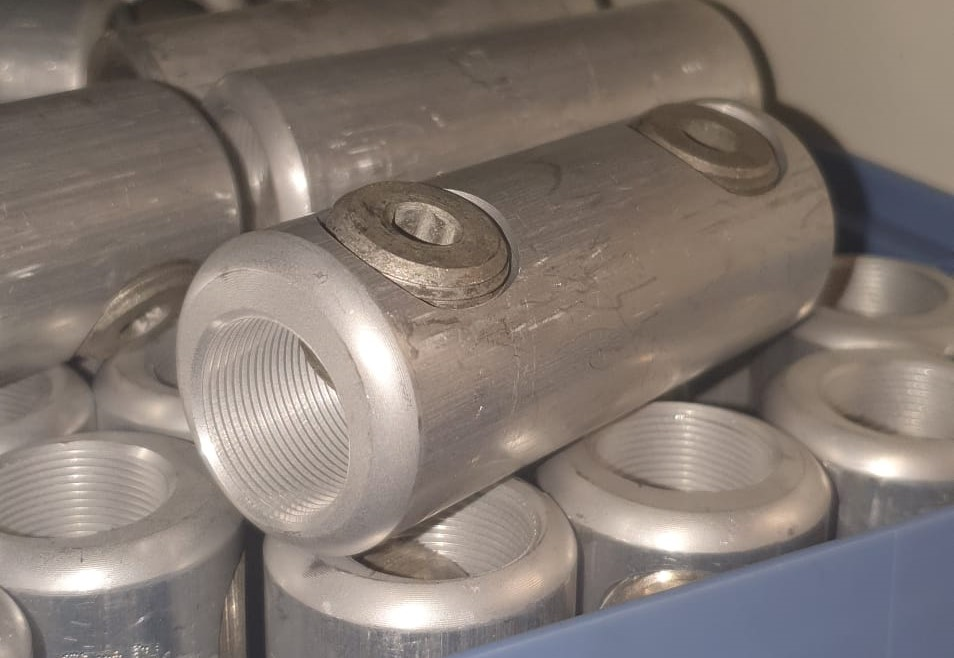
\includegraphics[width=0.98\linewidth]{images/Schraubverbinder}
\caption[Schraubverbinder]{Schraubverbinder Niederspannung}
\label{fig:Schraubverbinder}
\end{figure}
\\
Der auf dem Bild zu sehende Schraubverbinder, wird ausschließlich im Bereich der Niederspannung eingesetzt, da dieser bis zu einem maximalen Aderquerschnitt 
von 150 $\text{mm}^2$ und 1 kV maximale Spannung einsetzbar ist. Dies ist ausreichend, da im Niederspannungsnetz der TWS Netz GmbH ein Aderquerschnitt von 
max. 150 $\text{mm}^2$ eingesetzt wird. Dieser Aderquerschnitt, auch als Nennquerschnitt eines Kabels bezeichnet, gibt die dicke einer einzelnen Ader an, mit Hilfe 
der sichtbaren Fläche beim durchtrennen einer Ader. Meist kommt vor diese Angabe noch eine andere Zahl, welche angibt, wie viele Adern ein Kabel hat. Eine 
solche Bezeichnung sieht wie im folgenden Beispiel aus: 4x150 $\text{mm}^2$. Zur Installation werden die Schraubverbinder auf alle vier Adern eines Erdkabels des 
Typs NAYY geschraubt und anschließend mit separaten Schrumpfschläuchen isoliert, um einen Kurzschluss zwischen den Leitern zu verhindern. Dieser Erdkabeltyp 
besteht aus vier Aluminiumleitern, welche einzeln isoliert sind und durch eine zusätzliche Füllung zwischen Außenmantel und Aderisolierung vor Verdrehung 
geschützt werden.%cite 7.0
\\
Um den Außenmantel zu ersetzen, wird bei einer Verbindungsmuffe ein großer Schrumpfschlauch über beide Kabel abgeschrumpft, um das gesamte Muffenpaket zu 
schützen, wenn es in der Erde liegt. Das Muffenpaket definiert sich aus dem Bündel der vier Schraubverbinder einer Verbindungsmuffe, den abgemantelten Adern 
der Kabel und dem darüber abgeschrumpften Mantelschlauch. %cite 7 
\\
Die Verwendung von Aluminiumkabel sind im Stromnetz geläufiger, als die Verwendung von Kupferkabeln, da diese ein leichteres Gewicht aufweißen und Aluminium 
kosteneffizienter ist. Vergleicht man dieses Gewicht eines Aluminiumkabels des Typs NAYY mit einem Kupferkabel des Typs NYY, dann kommt man auf eine 
Reduzierung des Gewichts durch den Aluminiumleiter von ca. 3,5 Tonnen pro Kilometer Kabel. Der preisliche Unterschied des Kupferkabels in Verbindung mit dem 
geringfügigen kleineren Leitungswiderstand ist nicht wirtschaftlich genug, um dem im Vergleich stehende Aluminiumkabel stand zu halten.%cite 9 
\\
Dieser Leitungswiderstand kann berechnet werden, mit Hilfe des spezifischen Widerstandes, dem Querschnitt und der Länge des Kabels. Der spezifische Widerstand 
ist eine konstante Größe für unterschiedliche Materialien und kann in folgender Tabelle abgelesen werden.

\begin{table}[hbt]	
	\centering
	\renewcommand{\arraystretch}{1.5}
	\captionabove[Materialkonstanten]{Materialkonstanten \autocite{Weigerber.2018}}
	\label{tab:Materialkonstanten }
	\begin{tabular}{|c|c|c|c|c|}
        \hline
		\textbf{Material} & \textbf{Symbol} & \textbf{spez. Widerstand} & \textbf{spez. Leitwert} & \textbf{Temperaturkoeffizient}\\
        \textbf{} & \textbf{} & \textbf{in} $\mathbf{\frac{\Omega \cdot \textbf{mm}^2}{\textbf{m}}}$ & \textbf{in} $\mathbf{\frac{\textbf{m}}{\Omega \cdot \textbf{mm}^2}}$ & \textbf{in} $\mathbf{\frac{1}{^\circ \textbf{C}}}$ \textbf{oder} $\mathbf{\frac{1}{\textbf{K}}}$\\
		\hline 
		Aluminium   & \ce{Al}               &   0,028 &   36    & 0,004     \\
		\hline 
        Silber      & \ce{Ag}               &   0,016 &   63    & 0,004     \\
        \hline
        Kupfer      & \ce{Cu}               &   0,018 &   56    & 0,004     \\
        \hline
        Gold        & \ce{Au}               &   0,023 &   44    & 0,004     \\
        \hline
        Platin      & \ce{Pt}               &   0,11  &   9     & 0,002     \\
        \hline
        Eisen       & \ce{Fe}               &   0,125 &   8     & 0,005     \\
        \hline
        Manganin    & \ce{Cu, Fe, Mn, Ni}   &   0,4   &   2,5   & 0,00001   \\
        \hline
        Chromnickel & \ce{Cr, Ni, Fe}       &   1     &   1     & 0,00005   \\
        \hline
	\end{tabular} 
\end{table}
Anschließend kann mit Hilfe der folgenden Formel ein Leitungswiderstand für unterschiedliche Materialien, Querschnitte und Längen berechnet werden.
\begin{equation}
R_a=\frac{\rho \cdot l}{A}=\frac{l}{\kappa \cdot A}
\label{eqn:Leitungswiderstand}
\end{equation}
Dieser Muffentyp wird auch im Bereich der Mittelspannung verwendet, da es die beste Variante zur Verbindung zweier Kabel darstellt. Hier ist die Installation 
allerdings deutlich komplizierter, da die Verbindung höheren Spannungen standhalten und zudem auch noch besser isoliert werden muss, um Kurz- und Erdschlüsse 
zu vermeiden. Ein Erdschluss ist eine elektrische Verbindung zwischen stromführendem Leiter und der umliegenden Erde. Je nach Kabel Typ unterscheidet sich der 
Aufwand, um die Verbindungsmuffe zu installieren. Meist wird diese jedoch bei Kunststoffkabeln angewandt, welche drei einzelne Leiter eines bestimmten 
Querschnitts aufweisen. Ein solches Kabelbündel hat die Bezeichnung 3x1x300 mm$^2$ und sagt aus, dass es drei einzeln isolierte Leiter des Nennquerschnitts 
300 mm$^2$ sind. %Bild_MS_Kabel% 
Jedes einzelne Kabel benötigt somit eine eigene Muffe, welche nach Einhaltung der Anleitung installiert werden muss. Dies ist von enormer Wichtigkeit, da jede 
Produktionsreihe andere Vorgehensweisen zur Installation aufweisen kann und somit Fehler und Sicherheitsrelevante Probleme entstehen können. Dies betrifft 
vor allem die exakte Länge der abzumantelnden Bereiche und Schichten der Isolierung, da Mittelspannungskabel verschiedene Isolierungsschichten besitzen, um 
den Leiter zu schützen. Ein Kabel des Typs NA2XS(F)2Y hat \zB sieben Schichten um den Leiter herum. Dazu zählen drei leitfähige Schichten, welche dafür 
sorgen, dass die Spannung an die Isolierung geleitet wird und zwei Kunststoffisolierungsschichten. Die innere der beiden stellt eine Isolierung zwischen dem 
Leiter und Kupferdrahtschirm her und die äußere stellt den Mantel dar, welcher das Kabel hauptsächlich vor äußeren Einflüssen schützt. Der sogenannte 
Kupferdrahtschirm ist bei Mittespannungskabeln eine zusätzliche Erde und dient zudem auch noch zur Abschirmung elektrischer Magnetfelder. Diese Magnetfelder 
entstehen bei jedem stromdurchflossenen Leiter und müssen vor allem bei Mittelspannung eingedämmt werden. Um bei einer Verbindung zweier Leiter 
sicherzustellen, dass die Verbindung des Kupferdrahtschirmes besteht, muss dieser ebenfalls verbunden werden. Dies erfolgt meist durch einen kleinen 
Schraubverbinder. Der Aluminiumleiter selbst, wird durch einen großen Schraubverbinder, mit Hilfe von vier Schrauben verbunden. Diese Schrauben brechen an 
einem bestimmten Punkt von selbst ab, um immer ein ähnliches Drehmoment zu erreichen. Ein Drehmoment beschreibt die aufzuwendende Kraft bei einer Drehung 
einer Schraube. Nach installieren des Schraubverbinders, ist es wichtig jeglichen Freiraum mit beiliegendem Füllmaterial zu füllen, um jegliche 
Lufteinschlüsse zu vermeiden. Diese Lufteinschlüsse in einer Mittelspannungsverbindung würden zu Geräuschen im Isolator des nächstliegenden Schaltwerks führen 
und sind zu vermeiden. Anschließend wird ein Schrumpfschlauch, welcher für 20 kV geeignet ist über der Verbindung abgeschrumpft, um diese vor Kurzschlüssen zu 
schützen. Zuletzt ist es noch wichtig einen Mantelschrumpfschlauch über dem Paket aus Schraubverbinder und Kupferschirm abzuschrumpfen, um die gesamte Muffe 
vor äußeren Einflüssen zu schützen. Da Mittelspannungskabel drei dieser Kabel für die Phasen L1, L2 und L3 besitzen, muss dieser Prozess dreimal wiederholt 
werden um eine Verbindung herzustellen. Eine weitere Methode stellt die Gießharzmethode dar, in der als Isolator ein Harz verwendet wird, welches in eine Form 
gegossen und anschließend ausgehärtet wird. Dieses Harz besteht aus einer zwei teiligen chemischen Mischung, welche nach vermischen miteinander reagiert und 
zu einer aushärtenden Kunststoffmasse wird. Diese Masse ist letztendlich isolierend und schützt nach Aushärtung die Muffe vor äußeren Einflüssen. Diese Methode 
wird nur noch bei Abzweigmuffen verwendet, da dass Schrumpfverfahren deutlich schneller und einfacher anzuwenden ist.
\\\\
Im Mittel- sowie Niederspannungsbereich haben die Kabel eine Lebensdauer laut Hersteller von xx (glaube 30 Jahren). Im Erneuerungsprogramm der TWS Netz GmbH 
werden diese Kabelstrecken ersetzt. Dabei müssen Kabel mit verschiedenen Eigenschaften und Querschnitten verbunden werden. 
Die Kabelauftrennung findet ihre Anwendung bei Kabeln des Typs N(A)KBA, welche alle drei Adern in einem Kabel besitzen und für den Übergang auf einen aktuell 
verwendeten Kabeltypen, welcher im dreier Bündel vorhanden ist, erst aufgetrennt werden muss. Da ein Kabel des Typs N(A)KBA mit ölgetränktem Papier, einem 
Bleischirm und einem Jutemantel, heißt einem aus Pflanzen hergestelltem Stoff, isoliert ist, muss vor allem auf umweltgerechte Entsorgung und fachgerechtes 
Arbeiten unter der Benutzung von PSA geachtet werden. Zudem wird nach entfernen der Isolierung und auftrennen der einzelnen Adern eine abschrumpfbare 
Ölstoppkappe installiert, um austretendes Öl zu verhindern und weitere Schädigung der Umwelt einzudämmen. Da dieser Kabeltyp meist einen im Verhältnis sehr 
kleinen Nennquerschnitt hat, muss zudem eine Übergangsmuffe zum erhöhen des Kabelquerschnitts installiert werden. Diese Art der Muffe wird äquivalent zu 
einer Verbindungsmuffe installiert. Allerdings hat diese den entscheidenden Unterschied, dass der Schraubverbinder einschraubbare Plastikeinsätze hat, um auch 
kleinere Kabelquerschnitte zentriert einzuführen und festzuschrauben. Durch die Zentrierung ist gewährleistet, dass das Kabel immer mittig im Schraubverbinder 
liegt und nicht bei der Installation verrutscht. Diese Übergangsmuffen gibt es für verschiedene Kabeltypen und sind je nach Problemstellung auch mehrfach, \zB 
um einen Zwischenübergang von 95 mm$^2$ auf 185 mm$^2$ zu schaffen, um dann auf 300 mm$^2$ zu verbinden. Kabelverbindungsmuffen und Übergangsmuffen tragen im 
Mittelspannungsnetz einen wichtigen Anteil in der Versorgungssicherheit, da Sie für die Versorgung von Ust. verantwortlich sind und zur Erneuerung und 
Instandhaltung des Bestandsnetzes beitragen.
\\
Ein weiterer Muffentyp ist die Abzweigmuffe, welche ausschließlich im Niederspannungsnetz verwendet wird und nur in der Gießharzmethode verbaut wird. Diese 
Muffenart dient dazu eine Abzweigung des Stromkabels zu schaffen um beispielsweise einen Haushalt anzuschließen. Für die Montage einer Abzweigmuffe wird beim 
Bestandskabel lediglich der Mantel, heißt die äußere Isolierschicht entfernt, um die einzelnen Adern freizulegen. Um nun einen Abzweig zu schaffen, wird mit 
Hilfe einer Kabelabzweigklemme ein Kontakt zum Bestandskabel hergestellt. Diese Abzweigklemme hat spitzen, welche sich bei der Montage, also dem festschrauben 
der Klemme um die Adern, durch die Isolierung drücken und sich in den Aluminiumleiter hineintreiben. Durch diese Kontaktpunkte kann nun der Strom fließen und 
somit können auch die einzelnen Adern in der richtigen Zuordnung an diese Klemme angeschlossen werden. Zuletzt muss noch die entfernte Isolierung 
wiederhergestellt werden. Dies erfolgt durch eine Plastikform, welche um das Abzweigbündel montiert und abgedichtet wird, sodass in diese das Gießharz 
eingefüllt werden kann. Nach Aushärtung stellt dieser Schutz aus Gießharz die neue Isolierung dar und sorgt für einen Schutz der betroffenen Stelle. Diese 
Art der Muffe hat eine wichtige Bedeutung im Stromnetz, da man es mit Ihr flexibel erweitern kann und somit wenig Aufwand betreiben muss, um \zB neue Häuser 
an das Netz anzuschließen.
\\\\
Ein letzter Typ der auch zu den Kabelmuffen zählt, ist das Kabelende. Dieses gibt es in zwei verschiedenen Ausführungen, dem spannungsfesten und 
spannungsfreien Kabelende. Das spannungsfeste Kabelende wird verwendet, um unter Spannung stehende Kabelenden zu isolieren gegen Kurzschluss und zusätzlich 
zu schützen vor Korrosion oder Beschädigung im Erdreich. Ein Kabel, bzw. der metallische Leiter kann durch eintretende Feuchtigkeit oder dem 
Umgebungssauerstoff in der Erde korrodieren, heißt sich zersetzen oder verrosten. Dadurch kann dieser unbrauchbar werden und muss somit durch ein Kabelende 
geschützt werden. Ein Kabelende kann gezielt verlegt werden, wenn \zB bekannt ist, dass in geraumer Zeit das Netzgebiet an dieser Stelle erweitert wird oder 
es kann entstehen durch die Erneuerung alter Kabel. Hierbei wird das alte Kabel meist nicht komplett aus dem Erdreich entfernt und wird nur versiegelt durch 
ein Kabelende. So ist gewährleistet, dass das Erdreich durch evtl. austretende Öle geschützt ist und das Kabel nicht korrodiert. Steht das Kabel unter 
Spannung muss darauf geachtet werden, dass ein spannungsfestes Kabelende montiert wird. Dieses unterscheidet sich zum normalen Kabelende darin, dass jede 
Ader einzeln mit einer schrumpfbaren Plastiktülle versiegelt wird und somit ein Kurzschluss zwischen den Adern vermieden wird. Eine Plastiktülle ist ein 
Plastikschlauch, der an einem Ende verschlossen ist und wie eine Kappe über der Ader montiert wird. Um zusätzlich das austretende Öl von alten Kabeln zu 
stoppen und die offenen Adern bei \zB spannungsfesten Kabelenden zu schützen, wird eine Endkappe über dem gesamten Kabel abgeschrumpft. Diese Endkappe ist 
bei spannungsfreien Kabelenden ausreichend und benötigt keine zusätzlichen Adertüllen.
\\\\
Allerdings bringen diese Muffen auch Nachteile mit sich, denn sie stellen immer eine Schwachstelle im Netz dar. Kleinste Fehler in der Montage können dazu 
führen, dass die Isolierung nicht komplett wasserdicht ist und somit über die Zeit Wasser eintritt und die Muffe langsam kaputt geht. Dieses Wasser sorgt 
für kleinere Kurzschlüsse zwischen den Phasen, in denen zusätzlich Lichtbögen entstehen und den Leiter langsam schmelzen, bis dieser keinen Kontakt mehr hat. 
Deshalb muss die Anzahl der Muffen so gering wie möglich gehalten werden, um die Schwachstellen zu minimieren und somit eine Versorgungssicherheit 
herzustellen. 

\section{Die Bedeutung von Kabelmuffen im Stromnetz der TWS Netz GmbH}

Das Muffen von Kabeln im Nieder- und Mittelspannungsnetz stellt für Netzerweiterungen und -erneuerungen im Stromnetz der TWS Netz GmbH eine grundlegende 
Tätigkeit zur Erhaltung der Stromversorgung dar. Bei falscher Montage können diese zu Störquellen im Stromnetz führen und müssen ausgetauscht werden. Dies 
hat zur Konsequenz, dass die betroffenen Stromkunden für einen gewissen Zeitraum keinen Strom haben, was negative Auswirkungen auf das Image mit sich ziehen 
kann. Zudem möchte man den Kabelwiderstand so gering wie möglich halten, um Leistungsverluste durch Kabelwiderstände zu minimieren. Aber auch für den 
Umweltschutz sind \zB Übergangsmuffen sehr wichtig, da andernfalls Öl aus alten Kabeln in das Erdreich sickern und dieses belasten würde. Zudem sind diese 
auch wichtig, wenn verschiedene Kabelquerschnitte verbunden werden, da nur sie für einen reibungslosen Übergang sorgen. Je nach Problemstellung gibt es 
verschiedene Techniken zur Installation, zwischen denen man auswählen kann. Dazu zählen die Warmschrumpf- oder Gießharztechnik. Beide Techniken wurden 
individuell an praktischen Problemen, wie \zB Verbindungs-, Übergangs- und Abzweigmuffen angewandt. Zudem wurden die wichtigsten zu beachtenden Regeln 
erlernt, um jegliche Art der Kabelmuffe anwenden zu können.

\clearpage

\fi